\documentclass[conference]{IEEEtran}
%\IEEEoverridecommandlockouts
% The preceding line is only needed to identify funding in the first footnote. If that is unneeded, please comment it out.
\usepackage{cite}
\usepackage{amsmath,amssymb,amsfonts}
\usepackage{algorithmic}
\usepackage{graphicx}
\usepackage{textcomp}
\usepackage[table]{xcolor}
\usepackage{url}
\usepackage{hyperref}
%\usepackage{subcaption}
%\usepackage{subfig}
\usepackage{array}
\usepackage{multirow}
\usepackage{multicol}
\hypersetup{
	colorlinks = true,
	linkcolor = blue,
	anchorcolor = blue,
	citecolor = blue,
	filecolor = blue,
	urlcolor = blue
}	

\newcommand\MyBox[2]{
	\fbox{\lower0.75cm
		\vbox to 1.7cm{\vfil
			\hbox to 1.7cm{\hfil\parbox{1.4cm}{#1\\#2}\hfil}
			\vfil}%
	}%
}

\def\BibTeX{{\rm B\kern-.05em{\sc i\kern-.025em b}\kern-.08em
		T\kern-.1667em\lower.7ex\hbox{E}\kern-.125emX}}
\begin{document}
		\title{Comparing Parallel Sorting Algorithms on a High Performance Computing Cluster}
			\author{\IEEEauthorblockN{Benjamin Pierce}
			\IEEEauthorblockA{
				\textit{Department of Computer and Data Sciences}\\ }
			\and
			\IEEEauthorblockN{Alberto Safra}
			\IEEEauthorblockA{ 
				\textit{Department of Computer and Data Sciences}}
			\and
			\IEEEauthorblockN{Colin Causey}
			\IEEEauthorblockA{ 
			\textit{Department of Computer and Data Sciences}}
			\and
			\IEEEauthorblockN{Jason Richards}
			\IEEEauthorblockA{
				\textit{Department of Computer and Data Sciences}}}
	\maketitle
	
\begin{abstract}
Sorting is commonly viewed as the most fundamental problem in the study of algorithms. Some cited reasons for this are that a great many software applications use sorting for various reasons, and a great many algorithms use sorting as a subroutine \cite{cormen_introduction_2009}. 
Given its ubiquity, therefore, it is valuable to be able to solve the sorting problem efficiently. 
For this reason, many efficient sorting algorithms have been developed (e.g., mergesort, quicksort, heapsort). 
Given the asymptotic lower bound of $\Omega(nlog(n))$ for comparison-based sorting algorithms such as these, a natural route to take to achieve greater performance is parallel computing. 
In the interest of wanting to select the optimal sorting algorithm to run on a parallel computer, it is valuable to empirically compare the performance of various parallelized sorting algorithms. 
This is the aim of our research. 
We conduct an empirical analysis and comparison of various parallel sorting algorithms. 
The criteria for evaluation are (i) execution time and (ii) scalability. 
The research was conducted on Case Western Reserve’s high-performance computing (HPC) architecture. 
We implement multiple parallel sorting algorithms and execute them with variously sized and randomly permuted input arrays. The execution times are recorded for each run. 
Additionally, we will run the algorithms on a varying number of CPUs (e.g., one CPU, two CPUs, four CPUs) in order to assess their scalability.
After collecting the data, we performed data analysis and used it to compare the sorting algorithms. 
The comparison will facilitate making an informed choice about which sorting algorithm to use under various conditions (e.g., the number of CPUs available and the size of the input array).
\end{abstract}

\section{Introduction}
Sorting is a fundamental problem to be solved in many algorithms and applications.
Any algorithm that depends on having some ordering to the data will likely deal with sorting in some form, and even simple tasks like "find the top $n$ examples" are accomplished using sorts. 
Today's world of "Big Data" has led to an astronomical increase in the amount of computing power needed to efficiently process data.
As a result, parallel computing has become an important and necessary approach to solving computationally-intensive problems.
Parallel computing is a paradigm where computation is spread across many processors, working at the same time, rather then the usual sequential, processing method.
The processors used in parallel computation can be within a single node (as in multithreading and shared-memory parallel architectures) or they can be distributed across multiple nodes interacting with each other (as in message-passing architectures).
In order to take advantage of the performance increases enabled by parallel computing, parallelized versions of various sorting algorithms have been developed and studied. While theoretical analysis of parallel sorting algorithms is useful for understanding the asymptotic differences in the runtimes, determining and analysing the empirical performance of the algorithms on a specific computer architecture is valuable for making an informed choice about which algorithm to choose for that particular architecture and under various conditions (e.g., the number of CPUs available and the size of the input array to sort).
This study focuses on an emperical evaluation of multiple parallelized versions of popular sorting algorithms: Quicksort, Mergesort, Heapsort, and Insertion Sort, with a particular focus on Quicksort and Mergesort. The algorithms are parallelized with OpenMP so as to take advantage of multithreaded, shared-memory parallelism on Case Western Reserve's HPC Markov cluster.

\section{Background \& Theory}
As mentioned before, all comparison based sorts have an asymptotic lower bound of $\Omega(nlog(n)$. 
Indeed,  Mergesort, and Heapsort achieve a $O(nlog(n))$ upper bound as well, and Quicksort behaves as $O(nlog(n))$ in the average case. 
Insertion sort, as a less advanced algorithm, has a upper bound of $O(n^2)$, as does Quicksort. \cite{cormen_introduction_2009} 
However, Quicksort's upper bound is rarely the case, and tends to have smaller constant factors then either Mergesort or Heapsort. \cite{hoare_algorithm_1961} % TODO wrong cite
Additionally, each algorithm is constructed differently, and some are more amendable to parallelization than others. 
\subsection{Insertion sort}
Insertion sort is the simplest sorting algorithm discussed here. 
It works by iteratively building a sorted array one element at a time. 
That is, the algorithm loops through the list, creating a sorted and unsorted part, and insterting each element it encounters at the correct location. 
This proceduce is $O(n^2)$ worst case, but tends to perform quite well on small datasets, and better then other $O(n^2)$ sorts, such as bubble sort. \cite{knuth_art_nodate} 
For this reason, inserstion sort is often used as a subroutine in hybrid sorts like Timsort, where it is called when the size of a subarray is smaller then some threshold. \cite{auger_et_al:LIPIcs:2018:9467} 
Insertion sort can be parallelized % TODO in what way @Albert
\subsection{Mergesort}
Mergesort is a divide and conquer sort that recursively divides an array into subarrays, and merges them together such that each subarray is sorted. 
This procedure can be seen in Figure \ref{mrg}.  
The recursive invariant is that each returned subarray is sorted, which can be proved by induction, as an array of length 1 is already sorted by definition. \cite{cormen_introduction_2009} 
\begin{figure}[h]
	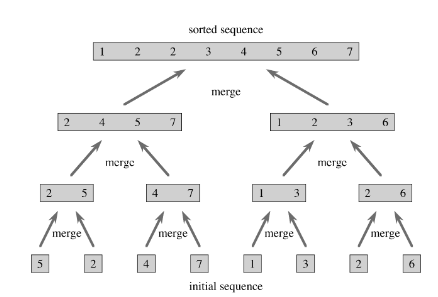
\includegraphics[width=6cm]{merge.png} 
	\caption{Mergesort diagram from \cite{cormen_introduction_2009}}
	\label{mrg}
\end{figure}
Mergesort has a time complexity of $O(nlog(n))$ in both the average and worst case, although constant factors can make it worse than Quicksort in practice. 
Mergesort is a natural candidate for parallelization; the divide and conquer nature of the algorithm is already suitable for this process. 
% TODO @Colin add detail on your implementation

\subsection{Heapsort}
Heapsort is another $O(n log(n))$ comparison sort. 
It, along with the heap data structure, was invented in 1964. \cite{forsythe_algorithms_1964}
Heapsort first turns the dataset into a max heap, which is a binary tree where each parent node is greater then its children. 
This process, called \textit{heapification}, is an $O(n)$ algorithum. 
Sorting is performed by repeatably popping the root node (the maximum value) and re-heapifying. 
This procedure takes advantage of the binary tree structure, and is worst case $O(n log (n))$ overall.  \cite{cormen_introduction_2009}
Unfortunately, Heapsort is a poor candidate for paralleization, as it does not partition into subarrays and depends on the root node being the absolute maximum. 
% TODO @Ben add detail on your implementation
\subsection{Quicksort}
The final sort discussed here is Quicksort, another $O(n log(n))$ comparison sort. 
Developed in 1961 \cite{hoare_algorithm_1961}, Quicksort is a partitioning sort that works by selecting a pivot element in an array and partitioning based on a comparison to the pivot, as shown in Figure \ref{qck}. 
\begin{figure}[h]
	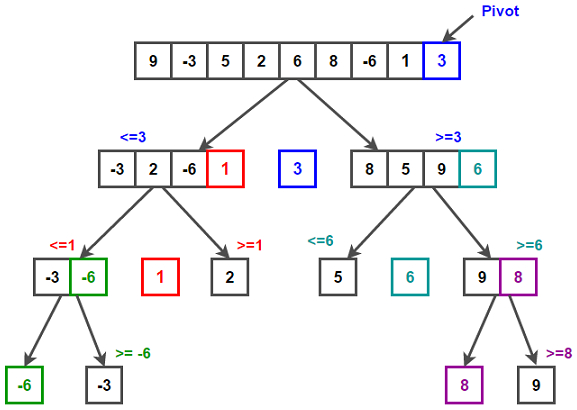
\includegraphics[width=6cm]{Quicksort.png} 
	\caption{Quicksort diagram. \href{https://www.techiedelight.com/quicksort/}{Source}}
	\label{qck}
\end{figure}
In particular, Quicksort is perhaps the most parallelizable sorting algorithm, and can achieve a linear speedup with few modifications. \cite{blelloch_programming_1996}
This is because each subarray can be sorted independently, and this leads to speedup. 
% TODO @Jason add detail on your implementation
\section{Methodology}
In this study, the OpenMP \cite{openmp08} API is used for parallization. 
It is an example of a fork-join methodology	, where each parallel thread forks off from a main thread, then, the results are joined back together. 
This is implemented into the C programming language via \textit{\#pragma} preprocessor directives. 
OpenMP is useful for obviously parallel cases, such as Mergesort and Quicksort, as the division of work is quite clear. 
% TODO add more OMP detail here.

This work utilizes Case Western Reserve University's Markov cluster, which runs on Intel Xeon x86\_64 Processors. 
Using the Simple Linux Utility for Resource Management \cite{yoo_slurm_2003} (SLURM), resources are allocated in batch mode, which enables repeatable, large scale experiments with the requested resources. 
% TODO do we need more detail?

\section{Results}
% TODO report results 
% TODO plot results as a function of array size
% TODO other results shit
\section{Conclusion}
% TODO these are what we expect to see...
As expected, the three $O(n log(n))$ algorithms perform better then Insertion sort. 
Due to the more parallel nature of Quicksort and Mergesort, these algorithms benefit more from parallization then the more sequential Heapsort. 
This is because the divide and conquer strategy is inherently more parallel, which should be taken into account when developing new algorithms to be run on parallel and distributed computing platforms. 
% TODO further findings from implementation
\bibliography{ref.bib}
\bibliographystyle{ieeetran}
\appendix
% TODO slap the code in here
\end{document}